\chapter{Results and Analysis}
\label{sec:rna}

% TODO: Include mention that this spans across 17 and 18 data.

Each of the GAN models described in Section \ref{sec:model_arch} were used to create artificial NIDS alert data.  Using the methods described in Section \ref{sec:meth} the fidelity of the learned model was analyzed. This analysis can be broken down into the following sections:

\begin{enumerate}
	\item Thorough Hyperparameter Search - Individual hyperparameters were tuned for each model to see their impact on histogram intersection. Top candidate values were selected for a full hyperparameter search where all combinations of hyperparameter values. The results are presented for both WGAN-GP and the improved WGAN-GPMI.
	
	\item Alert Fidelity - A subset of target IPs from both the CPTC'17 and CPTC'18 dataset were used for training WGAN-GP and WGAN-GPMI models. The results of these models were analyzed and visualized using histogram intersection and Jensen-Shannon Divergence.
	
	\item Alert Dependency - For the same subset of target IPs alert dependencies were identified by using drop in histogram intersection, entropy computation, and conditional probability tables.
	
	\item Output Modes Captured - The number of output modes captured by the model is comprised of two components. How many of the true output modes are output by the model. And how many output modes by the model do not occur in the ground truth. 

\end{enumerate}

\section{Thorough Hyperparameter Search}
\label{sec:search}
A two part hyperparameter search was employed to find optimal values for generating alerts from the CTPC datasets. First, individual parameters were tested in order to find several values which resulted in promising results. For each parameter value tested, the histogram intersection was computed for all possible feature value combinations. These values were then plotted against all other parameter settings results for WGAN-GP and WGAN-GPMI. Then, these values were taken and used for a full parameter sweep, which tested every possible combination of the parameter values available. Several candidate values were selected for each of the hyperparameters due to the unknown nature of hyperparameter interaction.

This two stage search was carried out twice, once for each of the GAN models presented in Section \ref{sec:model_arch}. The parameters tested included batch size, hidden dimension, learning rate, lambda, and number of epochs.

\subsection{Batch Size}
The batch size determines how many alert samples were fed into the model in parallel. Higher batch sizes can are more computationally intensive, but provide a better representation of the ground truth data distribution. Additionally, larger batch sizes reduce the number of steps required to complete a full epoch of training. 

The values tested for batch size were $\{10, 25, 50, 100, 150, 250, 500, 1000\}$. The intersection vs. parameter setting plots for WGAN-GP and WGAN-GPMI may be seen in Fig. \ref{fig:wgan_batch_size} and Fig. \ref{fig:gpmi_batch_size} respectively.

\begin{figure}[!htbp]
	\centering%
	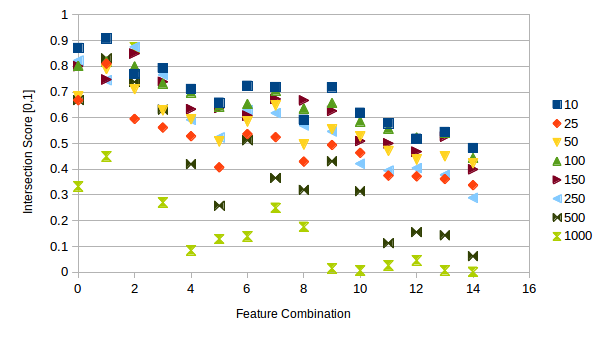
\includegraphics[width=\textwidth]{wgan_batch_size}
	\caption{
		All other hyperparameters were held constant at the following values: $epochs=180$, $learning\_rate=5e-5$, $hidden\_dimension=128$, $\lambda=0.1$
	}
	\label{fig:wgan_batch_size}
\end{figure}

\begin{figure}[!htbp]
	\centering%
	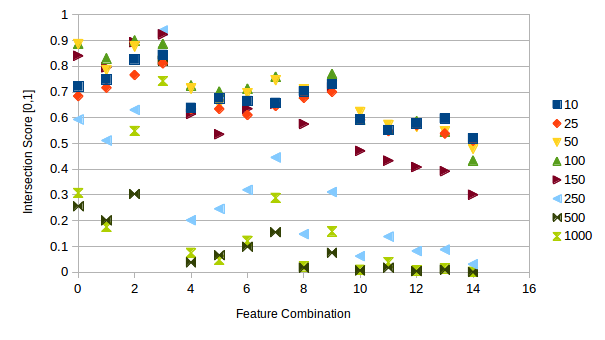
\includegraphics[width=\textwidth]{gpmi_batch_size}
	\caption{
		All other hyperparameters were held constant at the following values: $epochs=250$, $learning\_rate=5e-4$, $hidden\_dimension=128$, $\lambda=0.3$
	}
	\label{fig:gpmi_batch_size}
\end{figure}


% TODO: Analysis

\subsection{Hidden Dimension}
The hidden dimension size determines the number of hidden units available in each hidden layer. Higher hidden dimensions provide more learnable connections to the network allowing the network to complex approximations. On the other hand, larger hidden dimension sizes leads to potential overfitting and raises the computational complexity of training the network. 

The values tested for hidden dimension were $\{64, 128, 256, 384, 512\}$. The intersection vs. parameter setting plots for WGAN-GP and WGAN-GPMI may be seen in Fig. \ref{fig:wgan_hdim} and Fig. \ref{fig:gpmi_hdim} respectively. 


\begin{figure}[!htbp]
	\centering%
	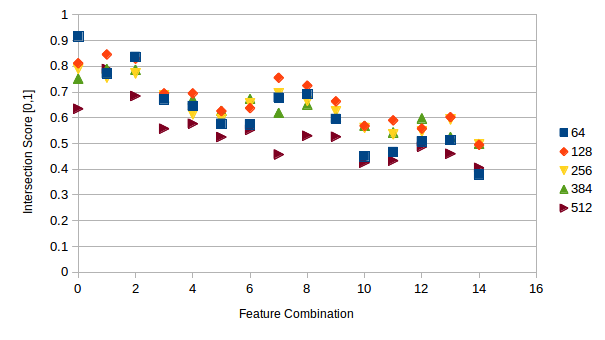
\includegraphics[width=\textwidth]{wgan_hdim}
	\caption{
		All other hyperparameters were held constant at the following values: $epochs=180$, $batch\_size = 100$, $learning\_rate=5e-5$, $\lambda=0.1$
	}
	\label{fig:wgan_hdim}
\end{figure}

\begin{figure}[!htbp]
	\centering%
	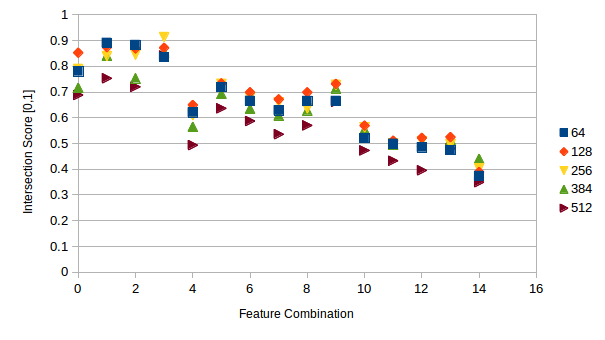
\includegraphics[width=\textwidth]{gpmi_hdim}
	\caption{
		All other hyperparameters were held constant at the following values: $epochs=250$, $batch\_size=100$, $learning\_rate=5e-4$, $\lambda=0.3$
	}
	\label{fig:gpmi_hdim}
\end{figure}

% TODO: Analysis

\subsection{Learning Rate}
The learning rate of the optimizer defines the base step size, weighted by the gradient of the loss, that is taken when adjusting parameter weights during training. A large learning rate converges quickly, but may overshoot the global optimum and never reach peak performance. A small learning rate won't overshoot the global optimum, however will take significantly longer to converge. Due to the categorical output of alert data and existing difficulty in optimizing GANs, small learning rates were tested. This allowed the network to be able to make fine tuned changes to network weights. Additionally, the ADAM optimizer was used, allowing for weight decay over time to modify the learning rate parameter. 


The values tested for hidden dimension were $\{1e-5, 5e-5, 1e-4, 5e-4, 1e-3\}$. The intersection vs. parameter setting plots for WGAN-GP and WGAN-GPMI may be seen in Fig. \ref{fig:wgan_lr} and Fig. \ref{fig:gpmi_lr} respectively. 

\begin{figure}[!htbp]
	\centering%
	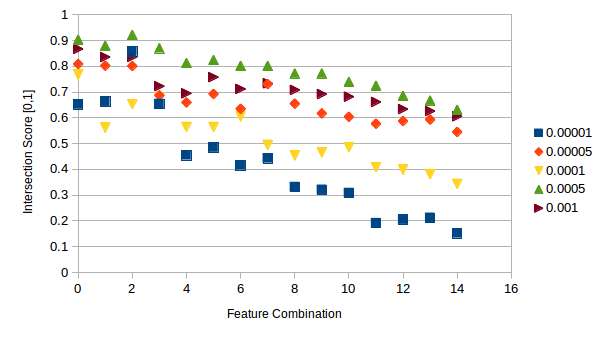
\includegraphics[width=\textwidth]{wgan_lr}
	\caption{
		All other hyperparameters were held constant at the following values: $epochs=180$, $batch\_size = 100$, $hidden\_dimension=128$, $\lambda=0.1$
	}
	\label{fig:wgan_lr}
\end{figure}

\begin{figure}[!htbp]
	\centering%
	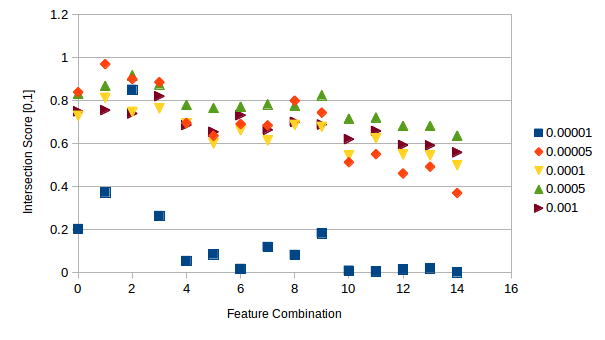
\includegraphics[width=\textwidth]{gpmi_lr}
	\caption{
		All other hyperparameters were held constant at the following values: $epochs=250$, $batch\_size=100$, $hidden\_dimension=128$, $\lambda=0.3$
	}
	\label{fig:gpmi_lr}
\end{figure}

% TODO: Analysis

\subsection{Lambda}
The lambda parameter was used as a coefficient to the gradient penalty term applied to the discriminator. The values tested for lambda were $\{0.05, 0.1, 0.2, 0.3, 0.4\}$. The intersection vs. parameter setting plots for WGAN-GP and WGAN-GPMI may be seen in Fig. \ref{fig:wgan_lam} and Fig. \ref{fig:gpmi_lam} respectively.

\begin{figure}[!htbp]
	\centering%
	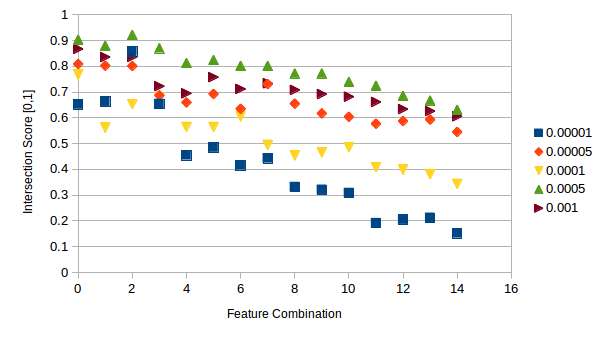
\includegraphics[width=\textwidth]{wgan_lr}
	\caption{
		All other hyperparameters were held constant at the following values: $epochs=180$, $batch\_size = 100$, $learning\_rate=5e-5$, $hidden\_dimension=128$
	}
	\label{fig:wgan_lam}
\end{figure}

\begin{figure}[!htbp]
	\centering%
	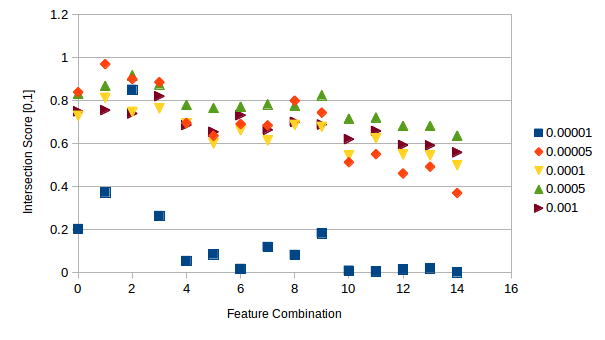
\includegraphics[width=\textwidth]{gpmi_lr}
	\caption{
		All other hyperparameters were held constant at the following values: $epochs=250$, $batch\_size=100$, $learning\_rate=5e-4$, $hidden\_dimension=128$
	}
	\label{fig:gpmi_lam}
\end{figure}

% TODO: Analysis

\subsection{Epochs}
The number of epochs determined how many times the network was exposed to the full dataset during training. Using a large number of epochs allows for the network to get more exposure to the ground truth distribution. However using a very large number of epochs can lead to the network memorizing the data. 

Due to the small size of the CPTC dataset, large values for epochs were tested. These values included $\{50, 100, 150, 200, 250\}$. The intersection vs. parameter setting plots for WGAN-GP and WGAN-GPMI may be seen in Fig. \ref{fig:wgan_epoch} and Fig. \ref{fig:gpmi_epoch} respectively. 

\begin{figure}[!htbp]
	\centering%
	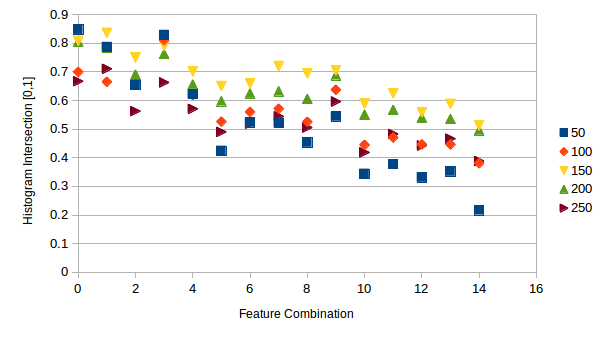
\includegraphics[width=\textwidth]{wgan_epoch}
	\caption{
		All other hyperparameters were held constant at the following values: $batch\_size = 100$, $learning\_rate=5e-5$, $hidden\_dimension=128$, $\lambda=0.1$
	}
	\label{fig:wgan_epoch}
\end{figure}

\begin{figure}[!htbp]
	\centering%
	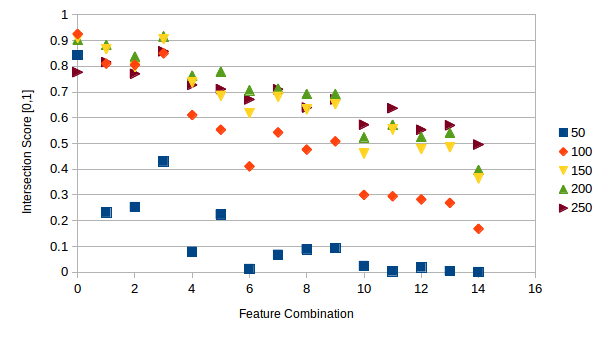
\includegraphics[width=\textwidth]{gpmi_epoch}
	\caption{
		All other hyperparameters were held constant at the following values: $batch\_size=100$, $learning\_rate=5e-4$, $hidden\_dimension=128$, $\lambda=0.3$
	}
	\label{fig:gpmi_epoch}
\end{figure}

% TODO: Analysis


\section{Alert Fidelity}
\label{sec:fidel}



\section{Alert Dependencies}
\label{sec:deped}



\section{Output Modes Captured}
\label{sec:output}


